\pagenumbering{arabic} 
\setcounter{page}{1}
\chapter{Cơ sở lí thuyết}
\section{Bài toán tối ưu}
Trong thực tế, ta thường gặp những vấn đề có nhiều cách giải quyết, một cách tự nhiên ta chọn cách giải quyết vấn đề một cách tối ưu nhất, chẳng hạn như nhanh nhất, tốn ít thời gian nhất hay mang lại hiệu quả kinh tế cao nhất... Đó được gọi là những bài toán tối ưu hóa.

Trong khoa học máy tính, bài toán tối ưu là bài toán tìm ra lời giải “tốt” nhất trong các lời giải khả thi. Tùy vào bài toán khác nhau sẽ định nghĩa độ tốt khác nhau, thường được gọi chung là hàm mục tiêu của bài toán. Có nhiều cách để phân chia lớp các bài toán tối ưu, một cách thường gặp là dựa vào tính chất của biến trong bài toán để chia bài toán thành hai loại: 
\begin{itemize}
    \item Bài toán tối ưu hóa liên tục: biến trong bài toán là biến liên tục. 
    \item Bài toán tối ưu hóa rời rạc (hay còn gọi là tối ưu hóa tổ hợp): biến trong bài toán là biến rời rạc.
\end{itemize}
Phần sau trình bày về hai dạng bài toán tối ưu trên. 

\subsection{Tối ưu hóa liên tục}
Theo \cite{convex_optimization}, dạng tiêu chuẩn của bài toán tối ưu hóa liên tục 
\[\begin{array}{lll}
    \mbox{minimize} & f(x)\\
    \mbox{subject to} & g_i(x) \leq 0 & i = 1, 2, ..., m\\
    \mbox{} & h_i(x) = 0 & i = 1, 2, ..., p\end{array}\]
Trong đó:
\begin{itemize}
    \item $f(x): R^n \rightarrow R$ là hàm mục tiêu cần đạt được 
    \item $g_i(x) \leq$ 0 được gọi là các ràng buộc bất đẳng thức 
    \item $h_i(x)$ = 0 là các ràng buộc đẳng thức 
    \item $m, p \in N$
\end{itemize}
Theo quy ước, dạng tiêu chuẩn xác định một bài toán cực tiểu hóa. Ta có thể định nghĩa bài toán cực đại hóa một cách tương tự.
\\Một ví dụ thường gặp của bài toán tối ưu liên tục là tối ưu giá trị của hàm số trong đoạn/khoảng cho trước.
\begin{figure}[H]
    \centering
    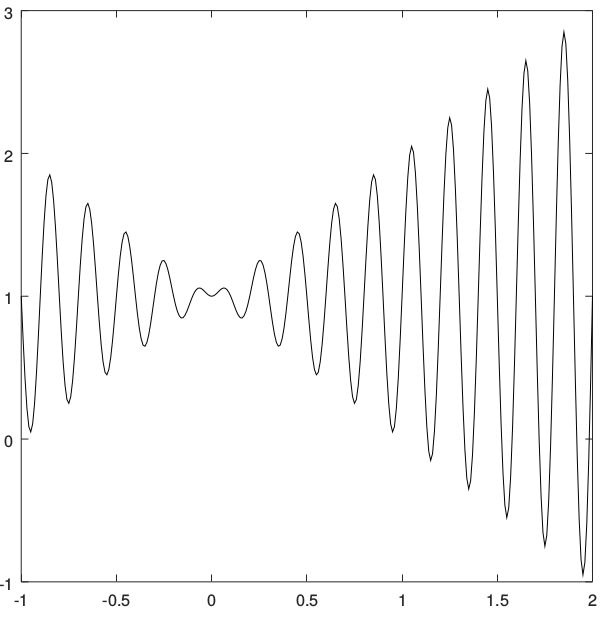
\includegraphics[width=0.8\linewidth]{picture/continuous_func.png}
    \caption{Đồ thị hàm $f(x) = x * sin(10\pi * x) + 1$}
\end{figure}
\subsection{Tối ưu hóa tổ hợp}
Như đã nêu ở trên, bài toán tối ưu tổ hợp là bài toán có biến quyết định nhận các giá trị rời rạc. Một cách tổng quát, một bài toán tối ưu tổ hợp có thể được định nghĩa bởi bộ ba ($S$, $f$, $\Omega$), trong đó $S$ là tập hữu hạn trạng thái (lời giải tiềm năng hay phương án), $f$ là hàm mục tiêu xác định trên $S$, $\Omega$ là tập các ràng buộc. Mỗi lời giải $s\in S$ thỏa mãn $\Omega$ được gọi là một lời giải chấp nhận được. Mục tiêu ở đây là tìm phương án $s^*$ tối ưu hóa toàn cục hạm mục tiêu $f$. Chẳng hạn với bài toán cực tiểu hóa thì $f(s^*) \leq f(s)$ với mọi phương án chấp nhận được $s$.
\\Ta đi đến một số bài toán tiêu biểu của lớp các bài toán tối ưu hóa tổ hợp. 
\\ \\\textbf{Bài toán người du lịch}
\\Nội dung bài toán: một người du lịch muốn tham quan $n$ thành phố $T_1, T_2, …, T_n$. Xuất phát từ một thành phố bất kì, người du lịch muốn đến tất cả các thành phố còn lại, mỗi thành phố đi qua đúng một lần rồi quay trở lại thành phố xuất phát. Gọi $C_{ij}$ là chi phí đi từ thành phố $T_i$ đến thành phố $T_j$, hãy tìm một hành trình thõa mản yêu cầu bài toán sao cho tổng chi phí di chuyển là nhỏ nhất.
\\Bài toán được mô hình hóa như sau 
\\Đầu vào:
\begin{itemize}
    \item $n$: số thành phố 
    \item $C_{nxn}$: ma trận kích thước n x n trong đó $c_{ij}$ là chi phí di chuyển từ thành phố i đến thành phố j
\end{itemize}
Đầu ra:
\begin{itemize}
    \item Hành trình đi qua n thành phố $T_{\pi(1)}, T_{\pi(2)}, …, T_{\pi(n)}$
\end{itemize}
Mục tiêu: tối thiểu hóa chi phí di chuyển  
\begin{equation}
    f = C_{\pi(1),\pi(2)}, C_{\pi(2),\pi(3)}, …, C_{\pi(n),\pi(1)} \rightarrow min
\end{equation}
Ràng buộc: mỗi thành phố chỉ đi qua một lần 
\begin{equation}
    \pi(i) \neq \pi(j) ~\forall ~1 \leq i, j \leq n
\end{equation}
Một cách lí thuyết, bài toán người du lịch sẽ có tất cả $n^n$ lời giải, tuy nhiên sẽ chỉ có $n!$ lời giải hợp lệ do ràng buộc mỗi thành phố chỉ được phép đi qua một lần. Nhiệm vụ tối ưu là tìm lời giải có tổng chi phí di chuyển nhỏ nhất trong $n!$ lời giải hợp lệ.
\\ \\\textbf{Bài toán cái túi}
\\Nội dung bài toán: một nhà thám hiểm cần đem theo một cái túi có trọng lượng không quá $b$. Có $n$ đồ vật có thể đem theo, đồ vật thứ $i$ có trọng lượng $a_i$ và giá trị sử dụng $c_i$ ($i$ = 1, 2, …, $n$). Hỏi nhà thám hiểm cần đem theo những đồ vật nào để tổng giá trị sử dụng là lớn nhất.

Một phương án của nhà thám hiểm có thể biểu diễn bởi một vector nhị phân có độ dài $n$: $z$ = ($z_1$, $z_2$, …, $z_n$), trong đó $z_i$ = 1 có nghĩa đồ vật thứ $i$ được mang theo và bằng 0 nếu ngược lại. 
\\Tổng giá trị các đồ vật đem theo là:
\begin{equation}
    f(x) = \sum_{i=1}^{n}c_ix_i
\end{equation}
Tổng trọng lượng đồ vật đem theo là:
\begin{equation}
    g(x) = \sum_{i=1}^{n}a_ix_i
\end{equation}
Đầu vào:
\begin{itemize}
    \item $n$ đồ vật 
    \item $b$ là trọng lượng tối đa có thể mang theo 
    \item $a = (a_1, a_2, ..., a_n): a_i$ là trọng lượng của vật $i$
    \item $c = (c_1, c_2, ..., c_n): c_i$ là trọng lượng của vật $i$
\end{itemize}
Đầu ra: 
\begin{itemize}
    \item Biến nhị phân $z = (z_1, z_2, ..., z_n): z_i$ = 1 khi vật $i$ được chọn 
\end{itemize}
Hàm mục tiêu: 
\begin{equation}
        f(x) = \sum_{i=1}^{n}c_ix_i \rightarrow max 
\end{equation}
Ràng buộc:
\begin{equation}
        g(x) = \sum_{i=1}^{n}a_ix_i \leq b 
    \end{equation}
\section{Các phương pháp giải bài toán tối ưu}
Giải bài toán tối ưu chính là đi tìm đáp án tốt nhất trong hàng loạt các đáp án khả thi của không gian lời giải. Có thể thu được lời giải tối ưu hàm mục tiêu trong không gian này nhưng đôi khi ta cũng chỉ có thể thu được lời giải “được coi là” tốt, liên quan đến hai khái niệm sau
\begin{itemize}
	\item Tối ưu toàn cục: lời giải tốt nhất thu được trong không gian lời giải của bài toán.
	\item Tối ưu cục bộ: lời giải tốt nhất trong một tập con của không gian lời giải.
\end{itemize}
Vậy vì sao lại dẫn đến trường hợp chỉ có kết quả “được coi là” tốt (tối ưu cục bộ)? Ta điểm qua các phương pháp giải bài toán tối ưu để làm rõ vấn đề này.
\subsection{Các phương pháp giải chính xác}
Như tên gọi, phương pháp giải chính xác cho bài toán tối ưu là phương pháp đem lại lời giải tốt nhất trong toàn bộ không gian lời giải của bài toán. Tiêu biểu là một số phương pháp sau.
\\ \\\textbf{Vét cạn}
\\Vét cạn là kĩ thuật với ý tưởng rất đơn giản: thử tất cả các phương án có thể của bài toán, kiểm tra liệu lời giải có vi phạm ràng buộc, kết luận phương án nào là tối ưu.
\\Phương pháp này có thể đảm bảo lời giải được tìm ra là tối ưu do đã xét mọi trường hợp có thể xảy ra, tuy nhiên lại gặp một trở ngại rất lớn: thời gian. Xét với một ví dụ đơn giản là bài toán người du lịch đã nêu ở trên, tập các lời giải khả thi là n!, chỉ cần tăng thêm một thành phố vào bài toán thì số lời giải khả thi đã tăng theo cấp số nhân, do đó phương pháp vét cạn hiển nhiên không thể áp dụng để giải bài toán này một cách hiệu quả.
\\ \\\textbf{Nhánh cận}
\\Ý tưởng của phương pháp nhánh cận đó là nếu ta dự đoán trước được những phương án có hàm mục tiêu chắc chắn tồi hơn hàm mục tiêu của phương án đã có trước đó, vậy ta không cần thử qua những phương án này nữa, nhờ đó thu hẹp được không gian tìm kiếm. Đây là một cải tiến của phương pháp vét cạn, cho phép tìm ra được lời giải nhanh hơn.
\\Trong phương pháp nhánh cận, ta sẽ xây dựng từng phần của lời giải cho đến khi tìm ra được lời giải tối ưu. Mô hình hóa lời giải thành vector $x = (x_1, x_2, …, x_n)$, giả sử tại bước $k$ ta đã xây dựng được $k$ thành phần của lời giải từ $x_1$ đến $x_k$, cần mở rộng thành phần $x_{k+1}$, nhưng khi đánh giá lại ta thấy tất cả các nghiệm mở rộng từ $x_k$ không có nghiệm nào có giá trị tốt hơn giá trị tối ưu ta đã biết tại thời điểm đó, vậy ta không cần mở rộng nữa, như vậy ta đã cắt bỏ đi một nhánh. 
\\Điều khó là phải đánh giá được các thành phần mở rộng, nếu đánh giá được tốt, thuật toán nhánh cận sẽ chạy nhanh hơn nhiều so với vét cạn. Tuy nhiên nhánh cận vẫn chỉ có thể áp dụng trong các bài toán có quy mô nhỏ.
\\ \\\textbf{Chia để trị}
\\Chia để trị là một phương pháp áp dụng cho các bài toán có thể giải quyết bằng cách chia nhỏ ra thành các bài toán con từ việc giải quyết các bài toán này. Sau đó lời giải của bài toán nhỏ được tổng hợp lại thành lời giải cho bài toán ban đầu.
Kĩ thuật chia để trị là cơ sở cho nhiều thuật toán hiệu quả, chẳng hạn như thuật toán sắp xếp, thuật toán nhân, thuật toán phân tích cú pháp. 
\\Kĩ thuật chia để trị thông qua ba bước:
\begin{itemize}
    \item Chia/tách nhỏ: tại bước này bài toán ban đầu được tách thành các bài toán con cho đến khi không thể tách được nữa, các bài toán con sẽ trở thành một bước nhỏ trong việc giải quyết bài toán lớn.
    \item Trị/giải quyết bài toán con: tại bước này sẽ tìm cách giải quyết bài toán con một cách cụ thể.
    \item Tổng hợp: khi đã giải quyết được các bài toán con, tổng hợp lại để có được lời giải của bài toán ban đầu.
\end{itemize}
\textbf{Quy hoạch động}
\\Được nhà toán học Richard Bellman phát minh vào năm 1953, quy hoạch động là một phương pháp mạnh mẽ tìm lời giải chính xác của các bài toán tối ưu. Phương pháp này thường dùng để giải các bài toán có cấu trúc con tối ưu và bài toán có các bài toán con gối nhau \cite{gtvlt}.
\\ \emph{Bài toán con gối nhau}, tương tự như chia để trị, quy hoạch động cũng chia bài toán ban đầu thành các bài toán con nhỏ hơn. Quy hoạch động được sử dụng khi các bài toán con này gọi đi gọi lại, kết quả của các bài toán con được lưu lại, do đó giảm thời gian tính toán.
Quy hoạch động sẽ không thể áp dụng được khi các bài toán con không gối nhau, do mỗi lần chia nhỏ, mỗi bài toán con chỉ được gọi một lần mà không được gọi lại.
\\ \emph{Cấu trúc con tối ưu} có nghĩa là các lời giải tối ưu cho các bài toán con có thể được sử dụng để tìm các lời giải tối ưu cho bài toán toàn cục. Ví dụ, đường đi ngắn nhất tới một đỉnh trong một đồ thị có thể được tìm thấy bằng cách: trước hết tính đường đi ngắn nhất tới đích từ tất cả các đỉnh kề nó, rồi dùng kết quả này để chọn đường đi toàn cục tốt nhất. Nói chung, ta có thể giải một bài toán với cấu trúc con tối ưu bằng một quy trình ba bước:
\begin{itemize}
    \item Chia bài toán thành các bài toán con nhỏ hơn.
    \item Giải các bài toán này một cách tối ưu bằng cách sử dụng đệ quy quy trình ba bước này.
    \item Sử dụng các kết quả tối ưu đó để xây dựng một lời giải tối ưu cho bài toán ban đầu.
\end{itemize}
Các bài toán con được giải bằng cách chia chúng thành các bài toán con nhỏ hơn, và cứ tiếp tục như thế cho đến khi ta đến được trường hợp đơn giản dễ tìm lời giải.
\\Quy hoạch động thường dùng thường dùng hai cách tiếp cận:
\begin{itemize}
    \item Top-down (từ trên xuống): chia bài toán ban đầu thành các bài toán con, giải và ghi nhớ lại lời giải của các bài toán con này phòng khi cần dùng. Đây là đệ quy và lưu trữ kết hợp với nhau.
    \item Bottom-up (từ dưới lên): tất cả các bài toán con có thể cần đến đều được giải trước, sau đó được dùng để xây dựng lời giải cho bài toán lớn hơn. Cách tiếp cận này tốt hơn về không gian bộ nhớ dùng cho ngăn xếp và số lời gọi hàm. 
\end{itemize}
Trên đây đã điểm qua một số phương pháp giải chính xác cho bài toán tối ưu hóa. Tuy nhiên đôi khi không thể tìm ra phương pháp giải chính xác cho bài toán tối ưu ngoại trừ vét cạn, hoặc có thể tìm được nhưng không gian lời giải bùng nổ cực kì nhanh khi kích thước bài toán tăng lên. Trong trường hợp đó sẽ cần sử dụng các phương pháp giải xấp xỉ để giải quyết bài toán.
\subsection{Các phương pháp giải xấp xỉ}
Đến nay đã có rất nhiều phương pháp giải xấp xỉ được đề xuất để giải quyết các bài toán tối ưu khác nhau. Dưới đây là một số ví dụ tiêu biểu.
\\ \\\textbf{Thuật toán tham lam }
\\Thuật toán tham lam giải quyết bài toán theo hướng luôn chọn tối ưu địa phương tại mỗi bước đi với hy vọng tìm được lời giải tối ưu toàn cục. Ví dụ với bài toán người du lịch, tại mỗi bước ta sẽ chọn thành phố tiếp theo bằng cách chọn thành phố gần nhất chưa đi qua.
Nói chung, thuật toán tham lam bao gồm năm phần:
\begin{itemize}
    \item Tập hợp các ứng viên để tạo ra lời giải. 
    \item Một hàm lựa chọn để theo đó chọn ứng viên tốt nhất để bổ sung vào lời giải.
    \item Một hàm khả thi, theo đó quyết định một ứng viên có phù hợp để đưa vào lời giải.
    \item Hàm mục tiêu, xác định giá trị của lời giải.
    \item Hàm đánh giá, chỉ ra khi nào lời giải hoàn chỉnh.
\end{itemize}
Giải thuật tham lam quyết định sớm hướng đi và không bao giờ xét lại các quyết định cũ. Đối với một số bài toán, đây có thể là một thuật toán không chính xác.
\\ \\\textbf{Tìm kiếm cục bộ}
\\Kĩ thuật tìm kiếm cục bộ đưa ra lời giải bằng cách tại mỗi bước cố gắng di chuyển đến lời giải láng giềng của lời giải hiện tại sao cho hàm mục tiêu được cải thiện. Các bước của kĩ thuật này như sau:
\begin{itemize}
    \item Xuất phát từ một lời giải bất kì. 
    \item Áp dụng một phép biến đổi lên lời giải hiện hành để thu được một lời giải tốt hơn. 
    \item Lặp lại phép biến đổi lên phương án hiện tại cho đến khi không thể cải thiện được nữa.
\end{itemize}
Do một phép biến đổi thường chỉ làm thay đổi một phần của phương án hiện tại để được một phương án mới nên được gọi là biến đổi địa phương, vì thế kĩ thuật này có tên tìm kiếm cục bộ.
\\ \\\textbf{Các thuật toán tiến hóa }
\\Thuật toán tiến hóa là tên gọi chung để chỉ lớp các thuật toán tìm kiếm và tối ưu hóa dựa trên nguyên lý tiến hóa tự nhiên. Một số thuật toán tiến hóa đã được công bố \cite{lap_trinh_tien_hoa}:
\begin{itemize}
    \item Quy hoạch tiến hóa: do D.B.Pogel đề xuất. Có thể diễn tả quy hoạch tiến hóa như sau: cho một lớp các phương pháp khả dĩ giải quyết được một (số) phần của vấn đề. Dựa vào quy luật tiến hóa, tìm một phương pháp liên hợp đủ khả năng giải quyết trọn vẹn vấn đề đó.
    \item Chiến lược tiến hóa: do T.Baeck, F.H.Hofmeister và H.P.Schwefel đề xuất. Thuật toán này dựa trên một số chiến lược ban đầu, tiến hóa để tạo ra những chiến lược mới phù hợp với môi trường thực tế một cách tốt nhất.
    \item Giải thuật di truyền: do J.H.Holland đề xuất, được D.E.Goldberg, L.Davis và Z.Michalevicz phát triển. Dựa trên quan niệm cho rằng quá trình tiến hóa tự nhiên là quá trình hoàn hảo nhất, hợp lý nhất và tự nó đã mang tính tối ưu \cite{lap_trinh_tien_hoa}.
\end{itemize}
Tiến hóa tự nhiên là một quá trình tối ưu. Đây có thể xem như một mệnh đề đúng, không chứng minh được, nhưng phù hợp với thực tế khách quan \cite{lap_trinh_tien_hoa}. Quá trình tiến hóa thể hiện tính tối ưu ở chỗ: thế hệ sau bao giờ cũng tốt hơn (phát triển hơn, hoàn thiện hơn) thế hệ trước. Tiến hóa tự nhiên được duy trì nhờ vào hai quá trình cơ bản: sinh sản và chọn lọc tự nhiên. Xuyên suốt quá trình tiến hóa tự nhiên, các thế hệ mới luôn được sinh ra để bổ sung thay thế thế hệ cũ. Cá thể nào phát triển hơn, thích ứng tốt hơn với môi trường sẽ tồn tại, ngược lại sẽ bị đào thải. Sự thay đổi môi trường là động lực thúc đẩy quá trình tiến hóa, đồng thời quá trình tiến hóa cũng làm thay đổi môi trường.
\\Các cá thể mới sinh ra nhờ sự lai ghép ở thế hệ cha mẹ. Một cá thể mới có thể mang các đặc tính của cha mẹ (di truyền) nhưng cũng có thể mang các đặc tính hoàn toàn khác (đột biến). Di truyền và đột biến có vai trò quan trọng như nhau trong quá trình tiến hóa, dù rằng đột biến xảy ra với xác suất nhỏ hơn nhiều so với di truyền. Các thuật toán tiến hóa tuy có những điểm khác biệt nhưng đều mô phỏng các quá trình cơ bản: lai ghép, đột biến, chọn lọc.
\begin{itemize}
    \item Lai ghép: là quá trình sinh ra cá thể mới bằng cách thừa hưởng các đặc tính từ cá thể cha mẹ.
    \item Đột biến: là hiện tượng cá thể con sinh ra mang một số tính trạng không có trong mã di truyền của cha mẹ.
    \item Chọn lọc: dựa trên cơ sở độ thích nghi của các cá thể, chọn ra các cá thể tốt phù hợp với môi trường.
\end{itemize}
\section{Giải thuật di truyền}
Giải thuật di truyền \cite{lap_trinh_tien_hoa} xuất hiện lần đầu vào năm 1962 trong công trình nghiên cứu về các hệ thống thích ứng của John Henry Holland, sau này được tiếp tục phát triển bởi chính học trò của ông là nhà khoa học David Edward Goldberg. Đến năm 1975, giải thuật di truyền chính thực được trình bày trong cuốn sách Adaptation in Natural and Artificial Systems (Thích nghi trong tự nhiên và trong các hệ thống nhân tạo).
\\Thuật giải di truyền sử dụng các thuật ngữ vay mượn của di truyền học. Ta có thể nói về các cá thể (hay kiểu gen, cấu trúc) trong một quần thể, những cá thể này có thể được gọi là chuỗi (hay nhiễm sắc thể). Điều này có thể gây lẫn lộn: mỗi tế bào của một cơ thể chủng loại đã cho mang một số những nhiễm sắc thể nào đó nhưng trong thuật giải di truyền, ta chỉ nói về những cá thể có một nhiễm sắc thể. Các nhiễm sắc thể được tạo thành từ các đơn vị (các gen) – biểu diễn trong một chuỗi tuyến tính. Mỗi gen kiểm soát một số đặc trưng.
\\Mỗi nhiễm sắc thể biểu diễn một lời giải của bài toán đang giải, một tiến trình tiến hóa được thực hiện trên một quần thể các các nhiễm sắc thể tương ứng với một quá trình tìm kiếm lời giải trong không gian lời giải. Tìm kiếm đó cần cân đối hai mục tiêu (có vẻ mâu thuẫn nhau): khai thác những lời giải tốt nhất và khảo sát không gian tìm kiếm, điểm mạnh của giải thuật di truyền là duy trì và xử lý một tập các lời giải (quần thể) trong suốt quá trình tìm kiếm, tạo được sự cân đối đáng kể giữa hai yêu tố trên. Nhờ việc duy trì nhiều lời giải này, giải thuật di truyền tìm kiếm trên nhiều điểm song song có khả năng leo lên nhiều cực trị cùng một lúc. Thông qua các toán tử của mình, giải thuật trao đổi thông tin giữa các cực trị với nhau, từ đó làm giảm thiểu khả năng giải thuật kết thúc tại các cực trị địa phương và bỏ qua mất cực trị toàn cục.
\\Tiếp theo đi vào chi tiết các bước của giải thuật di truyền.
\subsection{Mã hóa cá thể}
Công việc đầu tiên cần thực hiện khi giải bài toán bằng giải thuật di truyền là chọn cách biểu diễn cá thể. Mã hóa cá thể là việc ánh xạ các tham số của bài toán lên một chuỗi có chiều dài xác định, tùy theo từng bài toán cụ thể mà có các cách biêu diễn khác nhau sao cho phù hợp, thuận lợi khi giải toán. Đây là công việc cực kì quan trọng, một cách biểu diễn mã hóa cá thể tốt quyết định tới 50\% thành công của giải thuật.
\\Có nhiều cách mã hóa cá thể nhưng có hai cách biểu diễn thông dụng nhất là biểu diễn nhị phân và biểu diễn sử dụng hoán vị.
Với biểu diễn nhị phân, mỗi cá thể tương ứng với một chuỗi bao gồm các bit 0 và 1, ý nghĩa của các bit này phụ thuộc vào từng tính huống cụ thể. Đây là cách biểu diễn đơn giản và thông dụng nhất trong các cách biểu diễn.
\\Ví dụ trong bài toán cái túi được nêu ở trên, có một cách mã hóa cá thể đơn giản như sau: đánh thứ tự $n$ đồ vật từ 1 đến $n$, mỗi cá thể được biểu diễn bằng một xâu nhị phân độ dài $n$, bit thứ $i$ bằng 1 có nghĩa là đồ vật thứ $i$ được chọn cho vào túi và bằng 0 nếu ngược lại.
Trong biểu diễn hoán vị, mỗi cá thể tương ứng với một hoán vị của tập $n$ ký hiệu nào đó. Chẳng hạn với bài toán người du lịch đã được nêu ở trên, với $n$ thành phố, ký hiệu cho các thành phố lần lượt là $T_1, T_2, …, T_n$. Mỗi cá thể, sự mã hóa của lời giải sẽ là một danh sách hoán vị của $T_1, T_2, …, T_n$ biểu diễn lộ trình mà người du lịch đã đi qua. 
\subsection{Khởi tạo quần thể }
Như đã nêu ở trên, giải thuật di truyền duy trì và xử lí một tập các lời giải trong suốt quá trình tìm kiếm, khởi tại quần thể chính là quá trình sinh ra các cá thể một số lượng nhất định (kích thước quần thể).
\\Quần thể được khởi tạo ban đầu sẽ ảnh hưởng tới tốc độ của giải thuật và đôi khi là cả kết quả cuối cùng, vì vậy việc khởi tạo các cá thể ban đầu của quần thể cũng cần sử dụng phương pháp phù hợp với bài toán. Có hai cách khởi tạo thường gặp là khởi tạo ngẫu nhiên và khởi tạo heuristic.
\begin{itemize}
    \item Khởi tạo ngẫu nhiên: cá thể được sinh ra một cách ngẫu nhiên, miễn là đáp ứng được các ràng buộc của bài toán.
    \item Khởi tạo heuristic: dựa vào các kinh nghiệm đã có, ta khởi tạo tập các cá thể với hi vọng tập này có một khởi đầu tốt hơn nhằm nhanh chóng tìm ra lời giải.    
\end{itemize}
\subsection{Các toán tử di truyền }
Các phép lai ghép, đột biến được gọi chung là các toán tử di truyền, các toán tử này sẽ quyết định chiều hướng tiến hóa của quần thể, do đó để đảm bảo kết quả tốt, ta cần có các toán tử lai ghép và đột biến phù hợp.
\subsubsection{Lai ghép}
Quá trình lai ghép diễn ra bằng cách ghép một hay nhiều đoạn gen từ hai nhiễm sắc thể cha-mẹ để hình thành nhiễm sắc thể mới mang đặc tính cả cha lẫn mẹ. Các cá thể mới thừa hưởng các đặc tính tốt sẽ có khả năng sinh tồn mạnh hơn, nhờ đó duy trì nguồn gen tốt trong quần thể.
\\Một số phép lai ghép cơ bản: lai ghép một điểm cắt, lai ghép hai điểm cắt.
Trong lai ghép một điểm cắt, một điểm phân cách được chọn ra, khi đó phần nằm phía sau điểm phân cách này của hai cá thể cha mẹ được hoán đổi với nhau sinh ra hai con mới. Tương tự với phép lai ghép hai điểm cắt, có hai điểm phân cách được chọn, phần tráo đổi là phần nằm giữa hai điểm cắt. 
\\Tuy nhiên hai phép lai ghép trên phần lớn được áp dụng khi cách mã hóa cá thể là mã hóa nhị phân, với cách mã hóa cá thể khác (ví dụ mã hóa hoán vị), cá thể con sinh ra chưa chắc là một cá thể hợp lệ và do đó phép lai ghép coi như vô nghĩa. Trong trường hợp này cần áp dụng một số phép lai ghép khéo léo hơn.
\subsubsection{Đột biến}
Khác với đặc điểm của phép lai ghép là tận dụng nguồn gen tốt sẵn có trong quần thể, đột biến là quá trình tiến hóa khi một hoặc một số gen của cá thể con không được thừa hưởng từ gen của cha mẹ. Phép đột biến xảy ra với xác suất thấp hơn nhiều so với phép lai và có thể được mô tả như sau: 
\begin{itemize}
    \item Chọn ngẫu nhiên một cá thể trong quần thể.
    \item Giả sử độ dài mã hóa của cá thể là $n$, chọn một số $k$ ngẫu nhiên thỏa mãn $1 \leq k \leq n$, thay đổi gen thứ $k$ sao cho cá thể vẫn phù hợp.
    \item Trả cá thể này về quần thể để tham gia quá trình tiến hóa tiếp theo.
\end{itemize}
\subsection{Hàm thích nghi }
Hàm thích nghi phản ánh độ tương thích của cá thể với môi trường, hàm thích nghi có giá trị càng tốt chứng tỏ cá thể càng mạnh, là đối tượng phù hợp để giữ lại trong quá trình tiến hóa.
\\Có nhiều cách chọn hàm thích nghi khác nhau tùy vào bài toán, một cách chọn hàm thích nghi phổ biến là sử dụng luôn hàm mục tiêu trong mô hình bài toán đã đề ra.
\subsection{Chọn lọc}
Chọn lọc là quá trình loại bỏ các cá thể xấu và để lại những cá thể tốt. Một số phương pháp chọn lọc phổ biến như: 
\begin{itemize}
    \item Sắp xếp quần thể theo độ thích nghi, chỉ giữ lại các cá thể tốt nhất.
    \item Chọn lọc theo bánh xa Roullette: các cá thể được xếp vào một vòng tròn với độ rộng của cung tương ứng với độ thích nghi, quay vòng tròn bằng cách sinh ra một số ngẫu nhiên trong khoảng (0, 1) rồi chọn ra cá thể tương ứng.
\end{itemize}
\subsection{Điều kiện dừng của giải thuật}
Điều kiện được đưa ra để đảm bảo tính dừng của giải thuật. Thường giải thuật di truyền dừng lại sau một số thế hệ xác định hoặc dừng khi sau một số thế hệ không cải thiện được hàm mục tiêu của bài toán. Đây là một tham số của bài toán sẽ được chọn ra một cách phù hợp trong quá trình thực nghiệm.
\subsection{Đánh giá giải thuật di truyền}
Ưu điểm:
\begin{itemize}
    \item Nhanh hơn và tốn ít tài nguyên hơn so với tìm kiếm truyền thống trong một không gian tìm kiếm lớn.
    \item Đơn giản, nếu có cách mã hóa cá thể chuẩn xác và hàm mục tiêu đúng, ta có thể tìm được lời giải mà không cần thực hiện quá nhiều công việc phức tạp.
\end{itemize}
Nhược điểm: 
\begin{itemize}
    \item Đây không phải là một giải thuật hoàn chỉnh do không phải lúc nào giải thuật cũng tìm được lời giải phù hợp.
    \item Có thể bị mắc tại các cục bộ địa phương, mặc dù phép đột biến có thể giúp giảm thiểu trường hợp này nhưng làm giải thuật tiêu tốn nhiều thời gian hơn.
    \item Đôi khi khó để tìm được cách mã hóa cá thể.    
\end{itemize}
\section{Lý thuyết đồ thị}
\subsection{Các khái niệm cơ bản về đồ thị}
Lý thuyết đồ thị là một lĩnh vực nghiên cứu đã có từ lâu đời và có nhiều ứng dụng trong thế giới hiện đại. Những tư tưởng cơ bản của lý thuyết đồ thị được đề xuất vào những năm đầu của thế kỷ 18 bởi nhà toán học lỗi lạc người Thụy sỹ - Leonhard Euler. Chính ông là người đã sử dụng đồ thị để giải bài toán nổi tiếng về 7 cây cầu ở thành phố Konigsberg.
\\Đồ thị là cấu trúc rời rạc có tính trực quan cao, rất tiện ích để biểu diễn các quan hệ. Có thể kể đến một số ứng dụng thực tế của đồ thị như:
\begin{itemize}
    \item Có tiềm năng trong nhiều lĩnh vực do đồ thị có thể dùng để biểu diễn mối quan hệ, nghiên cứu quan hệ giữa các đối tượng là mục tiêu của nhiều lĩnh vực khác nhau.
    \item Ứng dụng trong mạng máy tính, mạng giao thông, mạng cung cấp nước, mạng điện, lập lịch, tối ưu hóa hệ thống, thiết kế mạch, quy hoạch phát triển,…
    \item Các ứng dụng khác: phân tích gen, trò chơi máy tính, chương trình dịch, thiết kế hướng đối tượng,…
\end{itemize}
Sau đây sẽ trình bày các khái niệm của đồ thị, nền tảng cho việc áp dụng lí thuyết đồ thị để giải quyết bài toán kéo dài thời gian sống của mạng cảm biến.
\subsection{Định nghĩa đồ thị}
Đồ thị là một tập các đối tượng được gọi là đỉnh, nối với nhau bởi các cạnh. Các loại đồ thị khác nhau được phân biệt bởi kiểu và số lượng cạnh nối. Ta định nghĩa các loại đồ thị như sau:

Đơn (đa) đồ thị vô hướng $G = (V, E)$ là cặp gồm 
\begin{itemize}
    \item Tập đỉnh $V$ là tập hữu hạn phần tử, các phần tử gọi là đỉnh 
    \item Tập cạnh $E$ là tập các bộ không có thứ tự dạng $(u, v), u, v \in E, u \neq v$
\end{itemize}
Đơn (đa) đồ thị có hướng $G = (V, E)$ là cặp gồm 
\begin{itemize}
    \item Tập đỉnh $V$ là tập hữu hạn phần tử, các phần tử gọi là đỉnh 
    \item Tập $E$ là tập các bộ có thứ tự dạng $(u, v), u, v \in E, u \neq v    $
\end{itemize}
\subsection{Đường đi và chu trình}
Định nghĩa: đường đi P độ dài n từ đỉnh u đến đỉnh v, trong đó n là nguyên dương, trên đồ thị $G = (V, E)$ là dãy
\begin{itemize}
    \item $P: x_0, x_1, …, x_n$
    \item Trong đó $u = x_0, v = x_n, (x_i, x_{i+1}) \in E, i = 0, 1, 2, …, n-1$
    \item Đỉnh $u$ gọi là đỉnh đầu, đỉnh $v$ gọi là đỉnh cuối của đường đi
\end{itemize}
Đường đi nói trên còn có thể biểu diễn dưới dạng dãy các cạnh: $(x_0, x_1)$, $(x_1, x_2)$, …, $(x_{n-1}, x_n)$.
\\Đường đi gọi là đường đi đơn nếu không có đỉnh nào bị lặp lại trên nó.
\\Đường đi gọi là đường đi cơ bản nếu không có cạnh nào bị lặp lại trên nó.
\\Nếu có đường đi từ đỉnh $u$ đến đỉnh $v$ thì ta nói đỉnh $v$ đạt đến được từ đỉnh $u$. Ta quan niệm rằng đỉnh v luôn đạt đến được từ chính nó.
\\Định nghĩa: đường đi cơ bản có đỉnh đầu trùng với đỉnh cuối ($u = v$) được gọi là chu trình.
Chu trình được gọi là đơn nếu như ngoại trừ đỉnh đầu và đỉnh cuối không có đỉnh nào bị lặp lại.
\section{Bài toán luồng cực đại }
\subsection{Các khái niệm}
Khái niệm mạng: mạng là đồ thị có hướng $G = (V, E)$
\begin{itemize}
    \item Có duy nhấtmột đỉnh $s$ không có cung đi vào gọi là đỉnh phát (nguồn) và duy nhất một đỉnh $t$ không có cung đi ra gọi là đỉnh thu (đích)
    \item Mỗi cung $e$ của $G$ được gắn với một số không âm $c(e)$ được gọi là khả năng thông qua của e
\end{itemize}
Luồng trong mạng: luồng $f$ trong mạng $G = (V, E)$ là phép gán số $f(e)$ cho mỗi cạnh $e$ ($f(e)$ được gọi là luồng trên cạnh $e$) thỏa mãn các điều kiện
\begin{enumerate}
    \item Hạn chế về khả năng thông qua 
    \begin{itemize}
        \item Với mỗi cung $e, 0 \leq f(e) \leq c(e)$
    \end{itemize}
    \item Điều kiện cân bằng luồng: với mỗi $v \neq s, t$
    \begin{itemize}
        \item $\sum_{e \in E^-(v)} f(e) = \sum_{e \in E^+(v)} f(e)$
    \end{itemize}
\end{enumerate}
Định nghĩa: giá trị của luồng $f$ là
\begin{itemize}
    \item $val(f) = \sum_{e \in E^-(s)} f(e) = \sum_{e \in E^+(t)} f(e)$
\end{itemize}
Định nghĩa: luồng trong mạng G được gọi là luồng cực đại nếu trong số tất cả các luồng trong mạng G
nó là luồng có giá trị lớn nhất. Bài toán tìm luồng cực đại trong mạng G được gọi là bài toán luồng cực
đại.
\\Định nghĩa: lát cắt là cách phân hoạch tập đỉnh $(S, T)$ sao cho $s \in S, t \in T$.
\\Khả năng thông qua $caps(S, T)$ của lát cắt $(S, T)$ là số:
\begin{itemize}
    \item $caps(S, T) = \sum_{e \in S \rightarrow T} c(e)$
    \item Trong đó: $S \rightarrow T := \{(v, w \in E: v \in S, w \in T)\}$
\end{itemize}
Lát cắt nhỏ nhất (hẹp nhất) là lát cắt với khả năng thông qua nhỏ nhất.
\\Bổ đề: giả sử $f$ là luồng, và $(S, T)$ là lát cắt. Khi đó giá trị luồng chảy qua lát cắt chính bằng giá trị luồng
\begin{itemize}
    \item $\sum_{e \in S \rightarrow T} f(e) - \sum_{e \in T \rightarrow S} f(e) = \sum_{e \in E^+(s)} f(e) = val(f)$
    \item Trong đó $S \rightarrow T := \{(v, w \in E: v \in S, w \in T)\}$ và $T \rightarrow S := \{(v, w \in E: v \in T, w \in S)\}$
\end{itemize}
Bổ đề: giả sử $f$ là luồng, còn $(S, T)$ là lát cắt, khi đó $val(f) \leq caps(S, T)$
Hệ quả: giả sử $f$ là luồng, còn $(S, T)$ là lát cắt. Nếu $val(f) = cap(S, T)$ thì $f$ là luồng cực đại, còn $(S, T)$ là lát cắt hẹp nhất.
\subsection{Định lý Ford - Fulkerson và thuật toán giải bài toán luồng cực đại}
Định lý Ford - Fulkerson: trong mạng bất kỳ, giá trị luồng cực đại luôn bằng khả năng thông qua của lát cắt nhỏ nhất.
\\ \textbf{Thuật toán Ford - Fulkerson:} 
\\Sau mỗi bước của thuật toán, các điều kiện sau cần được duy trì
\begin{itemize}
    \item $f(u, v) \leq c(u, v)$: luồng từ $u$ tới $v$ không vượt quá khả năng thông qua
    \item $f(u, v) = -f(v, u)$: ta duy trì cân bằng luồng 
    \item $\sum_f(u,v) = 0$: cho tất cả các nút ngoại trừ s và t. Lượng đi vào vào một nút bằng lượng đi ra khỏi nút đó. 
\end{itemize}
Điều này có nghĩa là một luồng đi qua mạng là một luồng hợp lệ sau mỗi bước lặp của thuật toán. Ta định nghĩa mạng thặng dư $G_f (V, E_f)$ là mạng với sức chứa $c_f (u, v) = c (u, v) - f (u, v)$ và luồng bằng không.

\begin{algorithm}[H]
    \SetKwData{START}{start}
    \SetKwData{MID}{mid}
    \SetKwData{END}{end}
    \SetKwData{Up}{up}
    \SetKwData{Energy}{E'}
    \SetKwData{ivar}{i}
    \SetKwData{jvar}{j}
    \SetKwData{TRUE}{True}
    \SetKwData{FALSE}{False}
    \SetKwData{varlone}{$l_1$}
    \SetKwData{varltwo}{$l_2$}
    \SetKwData{varlthree}{$l_3$}
    \SetKwFunction{MaxFlow}{MaxFlow}
    \SetKwFunction{FindConnect}{FindConnect}
    \SetKwInOut{Input}{Đầu vào}
    \SetKwInOut{Output}{Đầu ra}
    \Input{\\ Đồ thị $G = (V, E)$ với khả năng thông qua $c (u, v)$ \\Điểm phát s \\ Điểm thu t}
    \Output{\\Luồng $f$ từ $s$ đến $t$ sao cho $f$ có giá trị cực đại}
        \SetAlgoLined
        \BlankLine
        \Begin{
            $f(u, v) \leftarrow 0 ~\forall ~u, v$\\
            \While{tồn tại đường đi từ $s$ đến $t$ trong $G$}{
                Tìm một đường đi $u_1 , u_2 ,..., u_k$ với $u_1 = s, u_k = t$ sao cho $c_f (u_i , u_{i+1}) > 0$ \\
                Tìm $m = min (c_f (u_i , u_{i+1}))$ \\
                $f (u_i , u_{i+1}) \leftarrow f (u_i , u_{i+1} ) + m$ \\
                $f (u_{i+1} , u_i ) \leftarrow f (u_{i+1} , u_i ) - m$
            }
            \DecMargin{1em}
        }
        \caption{Thuật toán Ford - Fulkerson}      
\end{algorithm}
Đường đi trong $G_f (V, E_f)$ có thể tìm được bằng thuật toán tìm kiếm theo chiều rộng (breadth first search - BFS) hoặc tìm kiếm theo chiều sâu (depth first search – DFS).